\documentclass[a4paper, 12pt]{article}

% packages
\usepackage{amssymb}
\usepackage[fleqn]{mathtools}
\usepackage{tikz}
\usepackage{enumerate}
\usepackage{bussproofs}
\usepackage{xcolor}
\usepackage[margin=1.3cm]{geometry}
\usepackage{logicproof}
\usepackage{diagbox}
\usepackage{listings}
\usepackage{graphicx}
\usepackage{lstautogobble}
\usepackage{hyperref}
\usepackage{multirow}
\usepackage{tipa}
\usepackage{pgfplots}
\usepackage{adjustbox}

% tikz libraries
\usetikzlibrary{
    decorations.pathreplacing,
    arrows,
    shapes,
    shapes.gates.logic.US,
    circuits.logic.US,
    calc,
    automata,
    positioning,
    intersections
}

\pgfplotsset{compat=1.16}

\pgfmathdeclarefunction{gauss}{2}{%
  \pgfmathparse{1/(#2*sqrt(2*pi))*exp(-((x-#1)^2)/(2*#2^2))}%
}

\allowdisplaybreaks % allow environments to break
\setlength\parindent{0pt} % no indent

% shorthand for verbatim
% this clashes with logicproof, so maybe fix this at some point?
\catcode`~=\active
\def~#1~{\texttt{#1}}

% code listing
\lstdefinestyle{main}{
    numberstyle=\tiny,
    breaklines=true,
    showspaces=false,
    showstringspaces=false,
    tabsize=2,
    numbers=left,
    basicstyle=\ttfamily,
    columns=fixed,
    fontadjust=true,
    basewidth=0.5em,
    autogobble,
    xleftmargin=3.0ex,
    mathescape=true
}
\newcommand{\dollar}{\mbox{\textdollar}} %
\lstset{style=main}

% augmented matrix
\makeatletter
\renewcommand*\env@matrix[1][*\c@MaxMatrixCols c]{%
\hskip -\arraycolsep
\let\@ifnextchar\new@ifnextchar
\array{#1}}
\makeatother

% ceiling / floor
\DeclarePairedDelimiter{\ceil}{\lceil}{\rceil}
\DeclarePairedDelimiter{\floor}{\lfloor}{\rfloor}

% custom commands
\newcommand{\indefint}[2]{\int #1 \, \mathrm{d}#2}
\newcommand{\defint}[4]{\int_{#1}^{#2} #3 \, \mathrm{d}#4}
\newcommand{\pdif}[2]{\frac{\partial #1}{\partial #2}}
\newcommand{\dif}[2]{\frac{\mathrm{d}#1}{\mathrm{d}#2}}
\newcommand{\limit}[2]{\raisebox{0.5ex}{\scalebox{0.8}{$\displaystyle{\lim_{#1 \to #2}}$}}}
\newcommand{\limitsup}[2]{\raisebox{0.5ex}{\scalebox{0.8}{$\displaystyle{\limsup_{#1 \to #2}}$}}}
\newcommand{\summation}[2]{\sum\limits_{#1}^{#2}}
\newcommand{\product}[2]{\prod\limits_{#1}^{#2}}
\newcommand{\intbracket}[3]{\left[#3\right]_{#1}^{#2}}
\newcommand{\laplace}{\mathcal{L}}
\newcommand{\fourier}{\mathcal{F}}
\newcommand{\mat}[1]{\boldsymbol{#1}}
\renewcommand{\vec}[1]{\boldsymbol{#1}}
\newcommand{\rowt}[1]{\begin{bmatrix}
    #1
\end{bmatrix}^\top}
\DeclareMathOperator*{\argmax}{argmax}
\DeclareMathOperator*{\argmin}{argmin}

\newcommand{\lto}[0]{\leadsto\ }

\newcommand{\ulsmash}[1]{\underline{\smash{#1}}}

\newcommand{\powerset}[0]{\wp}
\renewcommand{\emptyset}[0]{\varnothing}

\makeatletter
\newsavebox{\@brx}
\newcommand{\llangle}[1][]{\savebox{\@brx}{\(\m@th{#1\langle}\)}%
  \mathopen{\copy\@brx\kern-0.5\wd\@brx\usebox{\@brx}}}
\newcommand{\rrangle}[1][]{\savebox{\@brx}{\(\m@th{#1\rangle}\)}%
  \mathclose{\copy\@brx\kern-0.5\wd\@brx\usebox{\@brx}}}
\makeatother
\newcommand{\lla}{\llangle}
\newcommand{\rra}{\rrangle}
\newcommand{\la}{\langle}
\newcommand{\ra}{\rangle}
\newcommand{\crnr}[1]{\text{\textopencorner} #1 \text{\textcorner}}
\newcommand{\bnfsep}[0]{\ |\ }
\newcommand{\concsep}[0]{\ ||\ }

\newcommand{\axiom}[1]{\AxiomC{#1}}
\newcommand{\unary}[1]{\UnaryInfC{#1}}
\newcommand{\binary}[1]{\BinaryInfC{#1}}
\newcommand{\trinary}[1]{\TrinaryInfC{#1}}
\newcommand{\quaternary}[1]{\QuaternaryInfC{#1}}
\newcommand{\quinary}[1]{\QuinaryInfC{#1}}
\newcommand{\dproof}[0]{\DisplayProof}
\newcommand{\llabel}[1]{\LeftLabel{\scriptsize #1}}
\newcommand{\rlabel}[1]{\RightLabel{\scriptsize #1}}

\newcommand{\ttbs}{\char`\\}
\newcommand{\lrbt}[0]{\ \bullet\ }

% colours
\newcommand{\violet}[1]{\textcolor{violet}{#1}}
\newcommand{\blue}[1]{\textcolor{blue}{#1}}
\newcommand{\red}[1]{\textcolor{red}{#1}}
\newcommand{\teal}[1]{\textcolor{teal}{#1}}

% reasoning proofs
\usepackage{ltablex}
\usepackage{environ}
\keepXColumns
\NewEnviron{reasoning}{
    \begin{tabularx}{\textwidth}{rlX}
        \BODY
    \end{tabularx}
}
\newcommand{\proofline}[3]{$(#1)$ & $#2$ & \hfill #3 \smallskip \\}
\newcommand{\proofarbitrary}[1]{& take arbitrary $#1$ \smallskip \\}
\newcommand{\prooftext}[1]{\multicolumn{3}{l}{#1} \smallskip \\}
\newcommand{\proofmath}[3]{$#1$ & = $#2$ & \hfill #3 \smallskip \\}
\newcommand{\prooftherefore}[1]{& $\therefore #1$ \smallskip \\}
\newcommand{\proofbc}[0]{\prooftext{\textbf{Base Case}}}
\newcommand{\proofis}[0]{\prooftext{\textbf{Inductive Step}}}

% ER diagrams
\newcommand{\nattribute}[4]{
    \node[draw, state, inner sep=0cm, minimum size=0.2cm, label=#3:{#4}] (#1) at (#2) {};
}
\newcommand{\mattribute}[4]{
    \node[draw, state, accepting, inner sep=0cm, minimum size=0.2cm, label=#3:{#4}] (#1) at (#2) {};
}
\newcommand{\dattribute}[4]{
    \node[draw, state, dashed, inner sep=0cm, minimum size=0.2cm, label=#3:{#4}] (#1) at (#2) {};
}
\newcommand{\entity}[3]{
    \node[] (#1-c) at (#2) {#3};
    \node[inner sep=0cm] (#1-l) at ($(#1-c) + (-1, 0)$) {};
    \node[inner sep=0cm] (#1-r) at ($(#1-c) + (1, 0)$) {};
    \node[inner sep=0cm] (#1-u) at ($(#1-c) + (0, 0.5)$) {};
    \node[inner sep=0cm] (#1-d) at ($(#1-c) + (0, -0.5)$) {};
    \draw
    ($(#1-c) + (-1, 0.5)$) -- ($(#1-c) + (1, 0.5)$) -- ($(#1-c) + (1, -0.5)$) -- ($(#1-c) + (-1, -0.5)$) -- cycle;
}
\newcommand{\relationship}[3]{
    \node[] (#1-c) at (#2) {#3};
    \node[inner sep=0cm] (#1-l) at ($(#1-c) + (-1, 0)$) {};
    \node[inner sep=0cm] (#1-r) at ($(#1-c) + (1, 0)$) {};
    \node[inner sep=0cm] (#1-u) at ($(#1-c) + (0, 1)$) {};
    \node[inner sep=0cm] (#1-d) at ($(#1-c) + (0, -1)$) {};
    \draw
    ($(#1-c) + (-1, 0)$) -- ($(#1-c) + (0, 1)$) -- ($(#1-c) + (1, 0)$) -- ($(#1-c) + (0, -1)$) -- cycle;
}

% AVL Trees
\newcommand{\avltri}[4]{
    \draw ($(#1)$) -- ($(#1) + #4*(0.5, -1)$) -- ($(#1) + #4*(-0.5, -1)$) -- cycle;
    \node at ($(#1) + #4*(0, -1) + (0, 0.5)$) {#3};
    \node at ($(#1) + #4*(0, -1) + (0, -0.5)$) {#2};
}

% RB Trees
\tikzset{rbtr/.style={inner sep=2pt, circle, draw=black, fill=red}}
\tikzset{rbtb/.style={inner sep=2pt, circle, draw=black, fill=black}}

% Samples
\tikzset{spos/.style={inner sep=2pt, circle, draw=black, fill=blue!20}}
\tikzset{sneg/.style={inner sep=2pt, circle, draw=black, fill=red!20}}

% Joins
\newcommand\ljoin{\stackrel{\mathclap{\normalfont\mbox{\tiny L}}}{\bowtie}}
\newcommand\rjoin{\stackrel{\mathclap{\normalfont\mbox{\tiny R}}}{\bowtie}}
\newcommand\ojoin{\stackrel{\mathclap{\normalfont\mbox{\tiny O}}}{\bowtie}}

\setcounter{MaxMatrixCols}{100}

% actual document
\begin{document}
    {\sc Computing $3^\text{rd}$ Year Notes} \hfill ~https://github.com/lin-e/imperial-revision~
    \rule{\textwidth}{0.1pt}
    \section*{CO331 - Network and Web Security \hfill (60015)}
        \subsection*{Week 1}
            \subsubsection*{Vulnerabilities}
                We define \textbf{vulnerabilities} as bugs or design flaws in software that can be exploited by attackers to compromise computers.
                These are taken advantage of by \textbf{exploits}, which are pieces of software.
                If it is unknown to the software vendor, it is referred to as a \textbf{zero day} (has not been disclosed to the public domain).
                \medskip

                \textbf{Advisories} are used to publicly disclose new vulnerabilities, issued by vendors or security companies.
                These are important for developers, sysadmins as well as regular users of the software, in order to keep up to date or patch systems.
                \medskip

                The \textbf{vulnerability reports} often vary in format.
                Bugs and systems can differ from each other, as well as researchers putting in varying levels of effort.
                Generally, the key information consists of the affected systems, descriptions, impact, proof of concept code, as well as proposed fixes.
                \medskip

                There are a number of approaches for when vulnerabilities are discovered;
                \begin{itemize}
                    \itemsep0em
                    \item \textbf{non-disclosure} \hfill keep the vulnerability secret
                        \smallskip

                        This is preferred by vendors who choose not to use resources to fix bugs (based on `security by obscurity'), or by parties intending to exploit it.
                        \medskip

                        An issue with hoarding vulnerabilities is the accidental release.
                        For example, \textit{WannaCry} used two exploits hoarded by the NSA - if this was disclosed, many more systems may have been patched.
                    \item \textbf{responsible disclosure} \hfill affected vendor decides when and what to release
                        \smallskip

                        This approach is preferred by software vendors, motivated by the idea that end users will not develop their own fixes.
                        However this can lead to a long duration between a discovery and fix.
                    \item \textbf{full disclosure} \hfill make details public
                        \smallskip

                        Eliminates any asymmetric information advantage attackers may have.
                        This method is preferred by security researchers, as well as the open source community.
                        However, it may affect users to attacks.
                        \medskip

                        The current approach, spearheaded by \textit{Google Project Zero}, is to give a window of time to vendors to fix vulnerabilities before it is publicly disclosed.
                \end{itemize}
            \subsubsection*{Malware}
                Malicious software can be characterised by infection vector;
                \begin{itemize}
                    \itemsep0em
                    \item \textbf{virus} \hfill malicious code copying into existing programs
                    \item \textbf{worm} \hfill replicates program over network or removable devices
                    \item \textbf{trojan / spoofed software} \hfill provides (or pretends to) useful service to act legitimate
                    \item \textbf{drive-by download} \hfill code executed by visiting malicious website
                \end{itemize}
                Another way to characterise malware is by purpose (malware often has multiple of these working together);
                \begin{itemize}
                    \itemsep0em
                    \item \textbf{rootkit} \hfill strongest, works at OS level (can hide itself)
                    \item \textbf{backdoor} \hfill allows attackers to connect over network
                    \item \textbf{RAT (remote access tool)} \hfill remote control
                    \item \textbf{botnet} \hfill recruit machine into botnet
                    \item \textbf{keylogger} \hfill logs keystrokes
                    \item \textbf{spyware} \hfill steals sensitive documents
                    \item \textbf{ransomware} \hfill blocks access to machine or data until ransom is paid
                    \item \textbf{cryptominer} \hfill uses system resources to mine cryptocurrency
                    \item \textbf{adware} \hfill displays advertisements
                \end{itemize}
                Malware can exist in several formats;
                \begin{itemize}
                    \itemsep0em
                    \item injected code added to a legitimate program
                    \item library loaded by a legitimate program
                    \item scripts run by application (such as macros in \textit{Microsoft Office})
                    \item standalone executable run by the user
                    \item code loaded in volatile memory (fileless malware) - without a file, detection can be difficult
                \end{itemize}
                Viruses can propagate in a number of ways, either by the attacker in the case of self-replication, or drive-by downloads, or installed by the user, either through social engineering or compromised certificates (in fake software updates).
                \medskip

                A virus can have varying privileges, either from the lowest level (in a rootkit, where it owns the machine), or have user privileges which can do limited damage.
                \medskip

                \textbf{APTs (Advanced Persistent Threats)} are used to reach high-value victims.
                These attacks are specific to the victim, often driven by a human.
                Decisions are made, depending on the specific configurations, and can involve compromising intermediate systems to reach the victim.
                Detection is avoided, with the use of rootkits to hide presence, as well as large datasets being exfiltrated over a long period of time.
                Avoiding detection is important as these attacks are often done over a long period of time, waiting for information to enter the system, as well as retaining access for later use.
                \medskip

                On the other hand, \textbf{botnets} are generic attacks, which aim to infect as many machines as possible.
                The idea is to infect many machines (bots) to allow an attacker (botmaster) to control them through a command-and-control server.
                The botnet can be used for the following;
                \begin{itemize}
                    \itemsep0em
                    \item \textbf{data theft} \hfill steal credit card numbers or passwords
                    \item \textbf{spam} \hfill less likely to be shut down, compared to single server
                    \item \textbf{DDoS} \hfill flood servers with requests
                    \item \textbf{brute-force} \hfill similar reasoning to spamming, passwords / credit card credentials
                    \item \textbf{network scanning} \hfill probing other hosts
                    \item \textbf{click fraud} \hfill generate advertising revenue from different sources
                    \item \textbf{cryptojacking} \hfill see above
                    \item \textbf{rental} \hfill botnets can also be rented out for use by others
                \end{itemize}
                Analysis can be performed on captured samples (to aid in detection or removal), obtained from cleaning up an infection or running \textbf{honeypots} (by willingly installing malware).
                Effects on storage, system settings and network traffic are often analysed in a virtual machine sandbox.
                However, it may be difficult to trigger malicious behaviour (since it may behave differently in a virtual environment).
                \medskip

                Detection can be performed by extracting signatures from analysed samples.
                \textbf{Static} signatures are sequences of bytes, typical of malware, and can be detected quite simply and quickly.
                However, this method is also easy to evade, where samples are artificially made different from each other, with \textbf{metamorphic} malware, or by the use of \textbf{crypting} services, which encrypt and obfuscate malware until it is no longer detected (FUD).
                \medskip

                On the other hand, \textbf{dynamic} signatures or behavioural analysis can be performed, where the host is monitored for patterns of actions typically performed by malware (such as reading data then sending data over a network).
                A way for this to be evaded is for the malware to mix malicious behaviour with legitimate behaviour.
                \medskip

                Current defences for malware include standard antivirus software, which scan existing and downloaded files for static signatures, as well as \textbf{end-point protection (EPP)}, which monitors the host for dynamic signatures.
                Browsers also now include blacklists which prevent access to pages known to be hosting phishing sites and malware.
                Network based protection can also be used.
                \medskip

                However, signatures and blacklists are both based on observed malware, therefore attackers have a window of opportunity before detection.
                As such, prevention is often the best strategy, such as educating humans to avoid direct installs.
                Software should also be updated and patched in response to disclosures; it is rare that zero-days are used in attacks, as they are difficult to find and expensive.
            \subsubsection*{Threat Modelling}
                Threat modelling can be used to guide decision making, by considering who the attackers are and their goals.
                We should also consider what attacks are likely to occur, and what assumptions the system relies on.
                \medskip

                Rather than performing the modelling on the code of the system itself, it's done on the model of the system, thus being free from implementation and deployment details.
                This allows us to identify better design implementations before the system is built, or can be used to guide the security review of a system after deployment.
                \medskip

                There are three key steps;
                \begin{enumerate}[1.]
                    \itemsep0em
                    \item model the system
                        \smallskip

                        This uses consistent visual syntax, to allow for multiple researchers to understand, as well as to build experience.
                        In this course, we focus on \textbf{system architecture}, rather than focusing on assets like passwords, credit card numbers, or focusing on attackers.
                        \medskip

                        \textbf{Data-flow diagrams (DFD)}s are used to depict the flow of information across components.
                        \textbf{Trust boundaries} help establish what principal controls what, and attacks tend to cross these boundaries.
                        \begin{center}
                            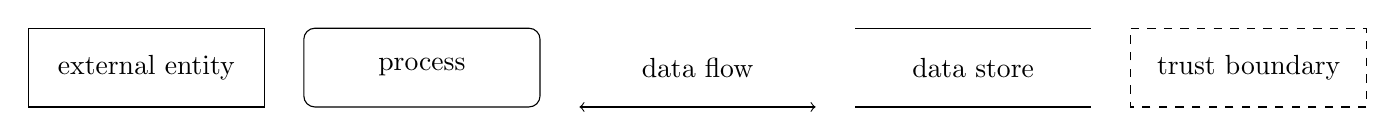
\begin{tikzpicture}
                                \begin{scope}[shift={(0, 0)}]
                                    \draw (0, 0) -- (3, 0) -- (3, -1) -- (0, -1) -- cycle;
                                    \node at (1.5, -0.5) {external entity};
                                \end{scope}
                                \begin{scope}[shift={(3.5, 0)}]
                                    \draw[rounded corners] (0, 0) -- (3, 0) -- (3, -1) -- (0, -1) -- cycle;
                                    \node at (1.5, -0.5) {process};
                                \end{scope}
                                \begin{scope}[shift={(7, 0)}]
                                    \draw (0, -1) edge[<->] (3, -1);
                                    \node at (1.5, -0.5) {data flow};
                                \end{scope}
                                \begin{scope}[shift={(10.5, 0)}]
                                    \draw (0, -1) -- (3, -1);
                                    \draw (0, 0) -- (3, 0);
                                    \node at (1.5, -0.5) {data store};
                                \end{scope}
                                \begin{scope}[shift={(14, 0)}]
                                    \draw[dashed] (0, 0) -- (3, 0) -- (3, -1) -- (0, -1) -- cycle;
                                    \node at (1.5, -0.5) {trust boundary};
                                \end{scope}
                            \end{tikzpicture}
                        \end{center}
                        For example, if two processes exist inside the same trust boundary, we generally don't need to be worried about attacks from one process to the other.
                        However, we do need to be concerned about any data flow arrows that cross the boundaries.
                    \item identify threats (STRIDE / attack trees)
                        \smallskip

                        For STRIDE, we ask what may go wrong in each element of a DFD;
                        \begin{itemize}
                            \itemsep0em
                            \item \textbf{s}poofing \hfill pretend to be something else
                            \item \textbf{t}ampering \hfill modifying without permission
                            \item \textbf{r}epudiation \hfill denying to have performed an action
                            \item \textbf{i}nformation disclosure \hfill revealing information without permission
                            \item \textbf{d}enial of service \hfill prevent system from providing a timely service
                            \item \textbf{e}levation of privilege \hfill achieve more than what is intended
                        \end{itemize}
                        Threats may belong to more than one of these categories, and threats should be document by writing risk-based security tests when possible.
                        \medskip

                        Another approach is to create an attack tree, where the root node represents the goal of the attack, or the target asset.
                        Children are the steps to achieve the goal, and the leaves are concrete attacks; by default, sibling nodes represent \textbf{sufficient} steps (only one needs to be satisfied), but special notation is used to represent \textbf{necessary steps} (where all need to be satisfied).
                        Note that the course uses lines between the arrows to denote necessary steps, however I will be using matching colours.
                        For example;
                        \begin{center}
                            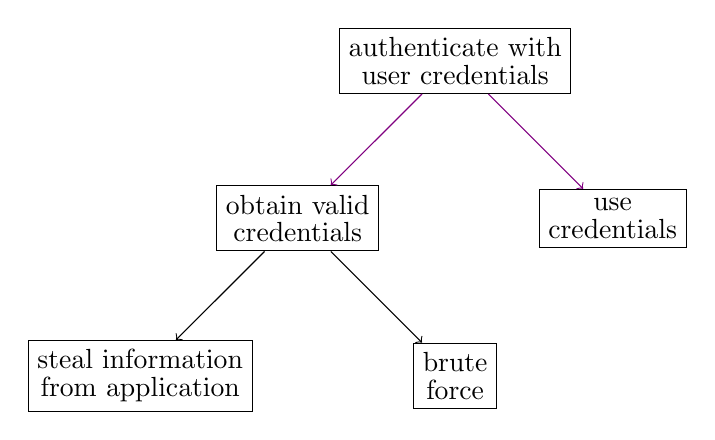
\begin{tikzpicture}[x=2cm, y=2cm];
                                \node[draw] (o) at (0, 0) {\shortstack{authenticate with\\user credentials}};
                                \node[draw] (ol) at (-1, -1) {\shortstack{obtain valid\\credentials}};
                                \node[draw] (or) at (1, -1) {\shortstack{use\\credentials}};
                                \node[draw] (oll) at (-2, -2) {\shortstack{steal information\\from application}};
                                \node[draw] (olr) at (0, -2) {\shortstack{brute\\force}};
                                \draw
                                (o) edge[->, violet] (ol)
                                (o) edge[->, violet] (or)
                                (ol) edge[->] (oll)
                                (ol) edge[->] (olr);
                            \end{tikzpicture}
                        \end{center}
                        This can also be represented in a textual format, where the root is a bullet point, and the necessary steps are `+', with the sufficient points being `-'.
                        \medskip

                        Attack trees are an alternative to STRIDE, for each element in a DFD, if the goal of an attack tree is relevant, the tree can be traversed to identify possible attacks.
                        Similarly, we can look at previously seen attack trees.
                        \medskip

                        It's important to focus on realistic threats.
                        The threats that should be considered depend on the system being modelled, the budget, and the value of what is being protected.
                    \item evaluate and address threads (DREAD / META)
                        \smallskip

                        The two main approaches for evaluating threats are qualitative (based on insight, experience, and expectations) and quantitative (based on some numerical score).
                        However, quantifying risk is difficult (and realistic parameters are hard to estimate), rare events are also hard to predict (and therefore hard to quantify).
                        \medskip

                        The DREAD methodology is a ranking from 5 to 15, developed by Microsoft;
                        \begin{center}
                            \begin{tabularx}{\textwidth}{|cl|X|X|X|}
                                \hline
                                & rating & high (3) & medium (2) & low (1) \\
                                \hline
                                \textbf{D} & damage potential & attacker can subvert full security system, get full trust authorisation, run as administrator, upload content & leaking sensitive information & leaking trivial information \\
                                \textbf{R} & reproducibility & attack can be reproduced every time and does not require a timing window & attack can be reproduced but only with a timing window and particular race situation & attack is difficult to reproduce, even with knowledge \\
                                \textbf{E} & exploitability & novice programmer could make the attack in a short time & skilled programmer could make the attack & extremely skilled person and in-depth knowledge to exploit every time \\
                                \textbf{A} & affected users & all users, default configuration, key customers & some users, non-default configuration & very small percentage of users, obscure feature \\
                                \textbf{D} & discoverability & published information explains the attack, vulnerability in most commonly used feature and is noticeable & vulnerability in seldom-used part of product, would take thinking to see malicious use & obscure bug, and users unlikely to work out damage potential \\
                                \hline
                            \end{tabularx}
                        \end{center}
                        After a thread is addressed, a response should be recommended;
                        \begin{itemize}
                            \itemsep0em
                            \item \textbf{m}itigate \hfill make threat harder to exploit
                                \smallskip

                                For example, if the threat was password brute-forcing, mitigations could require better passwords or locking accounts after some number of failed attempts.
                            \item \textbf{e}liminate \hfill remove feature exposed to threat
                            \item \textbf{t}ransfer \hfill let another party assume the risk
                                \smallskip

                                Continuing with the login scenario, we can use a third party login system.
                                The cost is that the third party has information about customers, and that legal responsibility may still remain (despite technological risk being transferred)
                            \item \textbf{a}ccept \hfill when other options are impossible or impractical
                                \smallskip

                                If someone was to guess the password on the first try, nothing can prevent it.
                                It's important to keep track that the threat remains active.
                        \end{itemize}
                        Responses should be documented, such as in a project issue tracker.
                \end{enumerate}
\end{document}